\section{问题二求解与分析}
\label{sec:q2}
\subsection{问题的描述与分析}
第二问延续第~\ref{sec:q1} 节的完整方案 $x=(\mathcal P,a,\boldsymbol\pi)$、总体任务执行时间 $C_q$ 和额外 COPY 字节 $D_q$，但重新界定执行任务：一个核心上的全部子图共同构成一个 Task。这个变化并未取消子图划分与核内顺序。子图仍规定算子的归核、局部先后与跨核边界；改变的是同核子图之间的状态能否延续，以及跨核交接的就绪条件。同一张量若由本核的后续子图使用，可以继续占据 L1 或 UB，不必因子图结束而立即写回。驻留时间也随之延长，可能触发自动换出；减少边界 COPY 并不保证周期一定缩短。

图~\ref{fig:q2_overview} 给出本问的求解脉络。首先按核心级 Task 重建交接与内存生命周期；随后沿用统一的完整评价和字典序接受准则，针对跨核通信、驻留峰值及可并行性提出不同候选。结果分析同时观察五核加速比、与第一问的逐图周期比、额外 COPY 变化和候选来源记录。前两问各自独立寻优，因而逐图比较的是两套执行规则下获得的方案表现，不能把差值全归因于 Task 语义变化。
\begin{figure}[htbp]
\centering
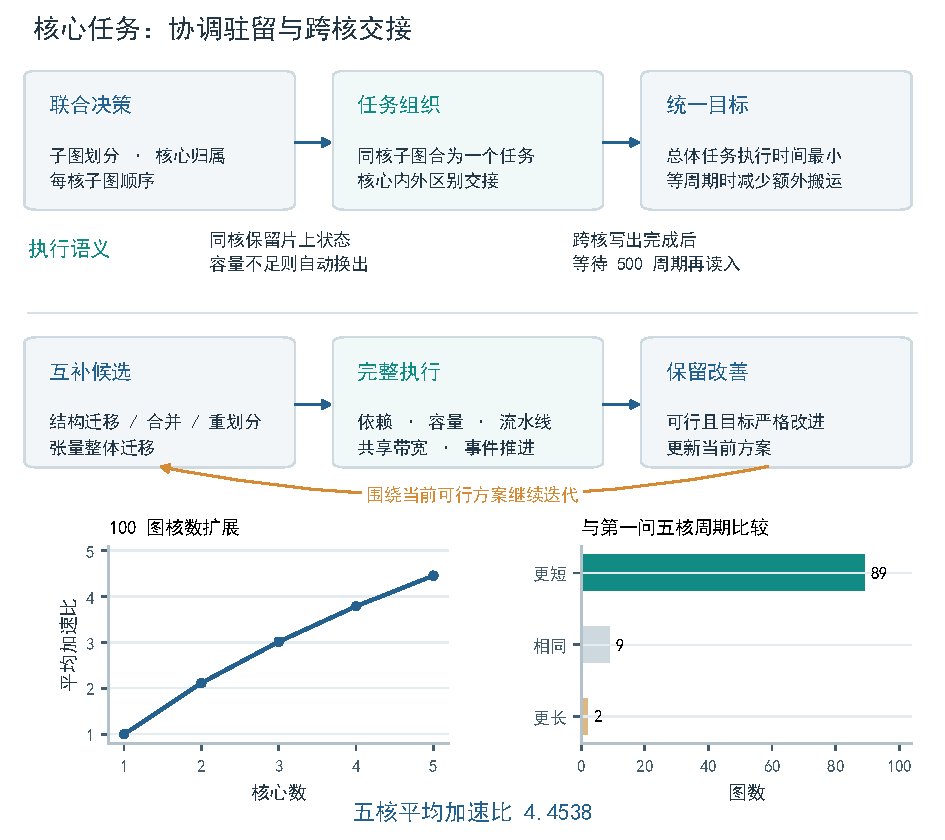
\includegraphics[width=\textwidth]{../求解/问题二/图片/q2_overview.pdf}
\caption{问题二的联合建模与迭代改进框架}\label{fig:q2_overview}
\end{figure}


\subsection{核心级任务的执行模型}
\subsubsection{同核驻留与跨核交接}
对核心 $k$，令 $\pi_k=(i_1,\ldots,i_{m_k})$，其全部子图属于同一 Task，任务标识为 $k$。同核相邻子图按方案顺序执行，但任务边界不在两者之间重复建立。若张量 $t$ 的生产者和后续消费者均位于 $k$，且执行过程未将相应缓冲换出，则消费者可读取本核驻留实例。图~\ref{fig:q2_task} 表示两类路径：同核复用沿着驻留状态传播，跨核依赖则先完成输出搬运，再进入目标核的读入队列。
\begin{figure}[htbp]\centering
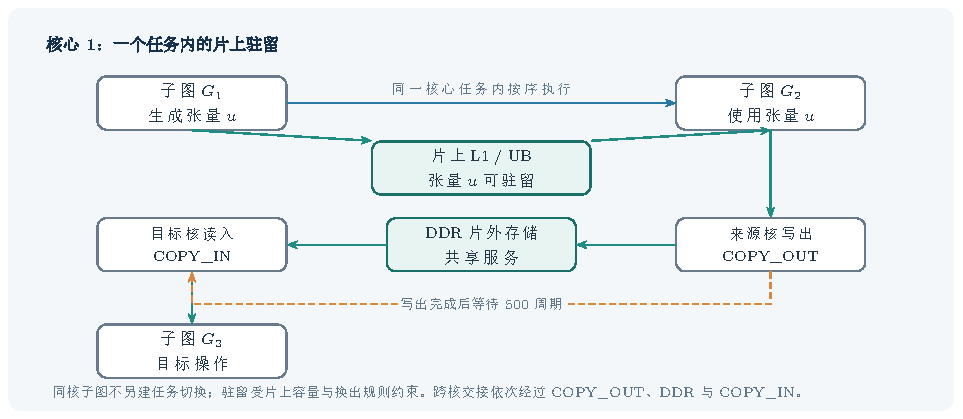
\includegraphics[width=\textwidth]{../求解/问题二/图片/q2_task.pdf}
\caption{核心级 Task 中的驻留与跨核交接}\label{fig:q2_task}
\end{figure}

对于跨核张量 $t$ 的一条交接，设相应 $\mathrm{COPY\_OUT}$ 完成于 $f_t^{\mathrm{out}}$，目标核的 $\mathrm{COPY\_IN}$ 开始于 $s_t^{\mathrm{in}}$。题设要求
\begin{equation}
 s_t^{\mathrm{in}}\ge f_t^{\mathrm{out}}+500.
 \label{eq:q2_handoff}
\end{equation}
若目标操作依赖多个跨核输入，则各输入分别满足式~\eqref{eq:q2_handoff}，其可启动时刻受最晚到达者约束；不能把多个 500 周期等待简单相加。同核路径不施加第一问的跨 Task 100 周期切换，也不虚构一次跨核读写。需要注意，式~\eqref{eq:q2_handoff} 只是释放读入的必要条件：$\mathrm{COPY\_OUT}$ 和 $\mathrm{COPY\_IN}$ 本身占用共享 DDR，目标核读入流水线、缓冲容量及其他依赖还可能继续推迟完成时刻。

本问与第一问的差别可在一个固定方案上写成执行映射的差别，而不改变优化变量：
\begin{equation}
 \mathcal E_2(G,x;\theta)\ne\mathcal E_1(G,x;\theta),\qquad
 \min_{x\in\mathcal F_2}^{\mathrm{lex}}\bigl(C_2(x),D_2(x)\bigr).
 \label{eq:q2_problem}
\end{equation}
这里 $\mathcal F_2$ 仍由无环、容量和完整执行可行性共同确定。由于两种映射重建的 COPY、缓冲生命周期和任务就绪时间不同，不能仅将第一问结果减去一个固定的任务切换常数来获得第二问周期。

\subsubsection{活跃集、自动换出与共享带宽}
同核跨子图驻留带来存储机会，也增加活跃区间。令 $\mathcal L_{k,r}(\tau;x)$ 表示在时刻 $\tau$，核心 $k$ 的存储区 $r\in\{\mathrm{L1},\mathrm{UB}\}$ 中仍占据空间的缓冲实例。每个时刻仍须满足第~\ref{sec:q1} 节式~\eqref{eq:capacity} 的容量约束；同一逻辑张量在不同核心形成的副本分别占空间。一个按子图顺序估计的峰值代理可记为
\begin{equation}
 M_r(x)=\max_{k,\tau}\sum_{b\in\mathcal L_{k,r}(\tau;x)}\operatorname{size}(b),
 \qquad r\in\{\mathrm{L1},\mathrm{UB}\}.
 \label{eq:q2_livepeak}
\end{equation}
式~\eqref{eq:q2_livepeak} 可提示哪些候选容易产生驻留压力，却不能代替实际分配结果：固定执行过程会按既定顺序、下一次使用位置和换出资格插入 Spill/Retrieve，峰值区间随事件时刻改变。当前操作正在使用的对象不能随意换出；候选也不能选择自由地址、重算张量或更改原始算子。联合调度与张量置换研究说明了驻留状态与片外访问的耦合\cite{A16}，而本题只借其状态分析来设计候选，不采用其自由地址和置换决策。合法拓扑顺序改变活跃集合及峰值存储的现象亦见于内存感知调度研究\cite{A17}；这里可调整的是子图划分、归核和核内子图顺序，不能改写原图。

额外 COPY 字节 $D_2(x)$ 汇总重建边界搬运及自动换出等题设计费项，却不是执行时间的线性代理。若多个核心同时提交 DDR 请求，第~\ref{sec:q1} 节式~\eqref{eq:bandwidth} 的共享服务率取决于当时在途请求数。局部减少字节，可能因为请求从非关键段移至关键段而并未缩短 总体任务执行时间；反过来，适度增加搬运，也可能提前释放依赖或让计算与通信重叠。因此，跨核 COPY 数、驻留峰值和计算负载在候选阶段用于解释与排序，最终保留仍由完整执行的 $(C_2,D_2)$ 判定。

\subsection{面向驻留与交接的候选改进}
\subsubsection{结构调整与张量事务}
第二问的基础与结构候选沿用第一问的完整方案表达，包括不同粒度的初始划分，以及围绕当前可行方案的迁移、交换、拆分与联合迁移。由第~\ref{sec:q1} 节的全局下界 $L$ 可报告当前结果仍可能改进的范围；固定候选下界 $L(x)$ 可筛去周期不可能优于当前方案的候选。核心级 Task 下，结构调整还有一项特殊价值：把生产者及消费它的子图放在同一核心，可能使跨核交接转为本核驻留读取。但共同归核会占用同一核心的计算 Pipe，并延长相应张量的生命期，所以它始终只是候选，而非必然改进。

对跨核使用频繁且字节数较大的张量，驻留来源先识别生产者和消费者涉及的完整子图集合，再取依赖与原有核序中需要一并移动的闭合子集，将这一组子图迁往某个已有归属核心。这样提出的是合法方案空间中的整体搬移，而不是切断一条依赖边，或令某张量在模型之外免费跨核。候选重新计算无环性、核心顺序及容量；实际 COPY 减少量和周期变化由完整评价取得。此类可行解上的局部迁移与多初值组织，在多处理器调度研究中有一般性的先例\cite{A42}，但其超步通信代价不用于本题的 DDR 事件评价。

另一个候选族保持原算子的核心归属，以依赖深度形成若干带，再按既有核心所有者划分子图。它试图把共享输入的使用收拢在较近的执行阶段，同时控制阶段内活跃集合；由于重新分组会改变局部并行性与缓冲寿命，候选并无单调收益保证。当图由相互独立的微小计算分量组成时，候选可把完整分量分配到核心，按容量估计限制每波同时展开的分量数，并将每波划成少量顺序阶段。这一“微波”宽度只是根据分量活跃峰值估计的提案尺度，不是满足真实容量的证明。两族候选分别适用于连接较多和较分散的结构，均需经过同一完整评价。

生产者前缀拆分也是方法库中的候选：当第一问的长子图阻碍跨 Task 张量提早释放时，可在保持依赖闭合的条件下拆出前缀。但该特定候选只对第一问的子图级 Task 启用，第二问不应把它作为已运行的改进来源。第二问跨核交接采用式~\eqref{eq:q2_handoff}，与第一问的任务完成等待不同；用第一问的释放逻辑替代本问评价会误判就绪时间。

\subsubsection{接受规则及质量解释}
所有来源都提交覆盖全部算子的完整 $x$，并在当前问题、核数及固定配置下接受执行检查。结构代理、活跃峰值和通信量只帮助产生候选，只有可行且 $(C_2,D_2)$ 字典序严格改善的结果才替换当前方案。第~\ref{sec:q1} 节命题3的归纳证明原样适用：已保留方案始终可行，目标序列单调不增。全局下界亦不因本问候选族改变而失效，因为其仅依赖保留的计算链、各类 Pipe 的总服务能力和已证明不可避的 DDR 流量。对五核结果，可计算 $1-L/C_2(x)$ 作为相对当前周期的最大可能减少比例；这是界的松紧，而不是已测得的算法误差或全局最优证明。

\subsection{实验结果与机制分析}
\subsubsection{核数扩展与逐图周期}
按式~\eqref{eq:speedup} 对每图先求相对原始整图单核的加速比，再在 100 图上取算术平均。表~\ref{tab:q2_mean} 与图~\ref{fig:q2_mean} 给出第二问随核心数变化的结果。一至五核的平均加速比分别为 $1.0000$、$2.1168$、$3.0153$、$3.7868$ 和 $4.4538$；五核中位数为 $4.7143$。四核升至五核的平均增量仍为 $0.6670$，但低于二核升至三核的 $0.8985$。核心级 Task 减少同核边界代价后，关键依赖链、各类计算 Pipe 的负载和共享 DDR 仍限制进一步并行。
% 由求解/规范化数据/combined/means.csv 生成；逐图加速比的算术平均。
\begin{table}[htbp]
\centering\small
\setlength{\tabcolsep}{5pt}
\begin{tabular}{rrrrrr}
\toprule
核心数 & 样本数 & 平均加速比 & 中位加速比 & 最小加速比 & 最大加速比 \\
\midrule
1 & 100 & 1.0000 & 1.0000 & 1.0000 & 1.0000 \\
2 & 100 & 2.1168 & 2.0189 & 1.5706 & 3.6533 \\
3 & 100 & 3.0153 & 3.0064 & 1.7941 & 5.4726 \\
4 & 100 & 3.7868 & 3.9421 & 1.9552 & 7.0716 \\
5 & 100 & 4.4538 & 4.7143 & 1.9919 & 8.7768 \\
\bottomrule
\end{tabular}
\caption{问题二各核数逐图加速比统计}\label{tab:q2_mean}
\end{table}

\begin{figure}[htbp]\centering
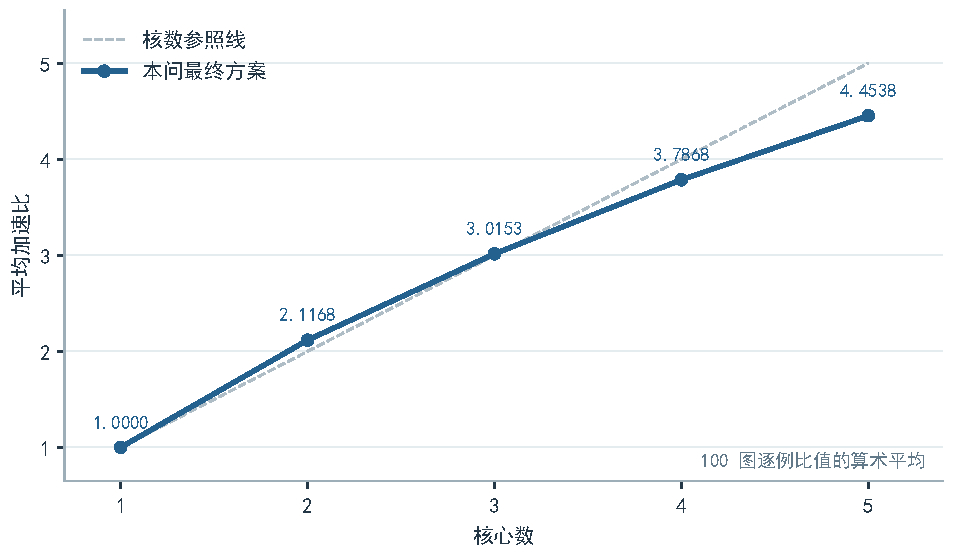
\includegraphics[width=.90\textwidth]{../求解/问题二/图片/q2_mean.pdf}
\caption{第二问各核数平均加速比}\label{fig:q2_mean}
\end{figure}

五核逐例加速比介于 $1.9919$ 和 $8.7768$，有 1 图低于 2，22 图高于 5。超过五倍并不表示硬件提供超过五核的计算吞吐：与原始单核参考相比，重新划分、核内顺序、搬运和自动换出同时变化，基线并非只少了四个核心。五核周期的全局下界与当前结果所给相对差距上界，逐图平均为 $0.2462$；其中 6 图的界在 $1\%$ 以内。其余图的界较松，既不能宣称已经最优，也不能把界宽全算作算法损失。

图~\ref{fig:q2_distribution} 将同一批图的第一、二问五核加速比放在共同尺度上，并保留逐图点。第二问的分布整体向较高加速比移动，但仍有长尾与个别反例。为避免把两个不同基线混入比较，逐图再定义
\begin{equation}
 R_i=\frac{C_{i,1,5}}{C_{i,2,5}},\qquad i=1,\ldots,100.
 \label{eq:q2_pairratio}
\end{equation}
由于两问都以相同的 $T_{i,0}$ 定义加速比，$R_i$ 亦等于同图第二问加速比除以第一问加速比。100 图中 $R_i>1$ 有 89 图，$R_i=1$ 有 9 图，$R_i<1$ 有 2 图；比值均值 $1.1728$、中位数 $1.0913$。这说明核心级 Task 的最终方案通常更快，但这些方案分别搜索，式~\eqref{eq:q2_pairratio} 不是保持 $x$ 不变的任务语义消融。
\begin{figure}[htbp]\centering
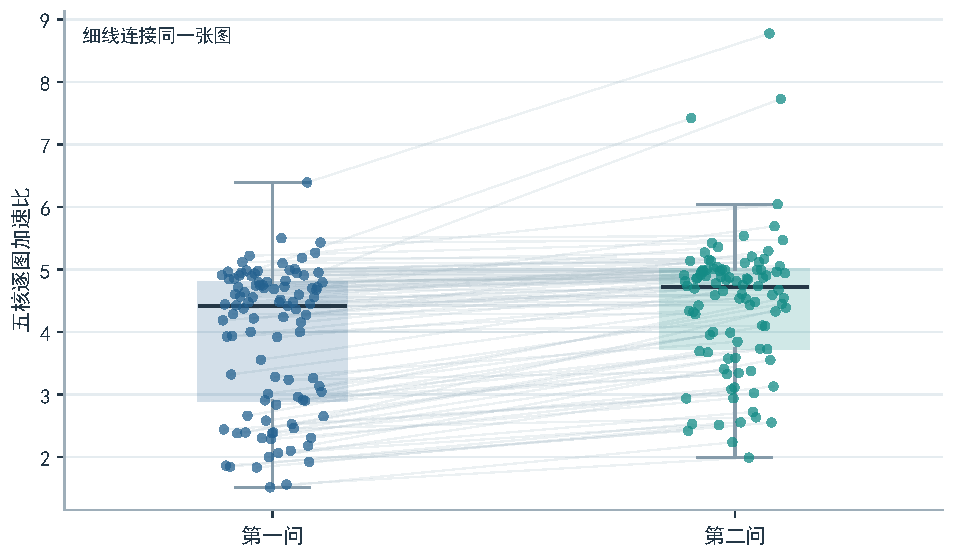
\includegraphics[width=.94\textwidth]{../求解/问题二/图片/q2_distribution.pdf}
\caption{五核逐图第一、二问加速比分布}\label{fig:q2_distribution}
\end{figure}

\subsubsection{COPY 量、驻留压力与反例}
第二问五核额外 COPY 字节的均值为 $8094619.10$ B，中位数为 $1310458$ B，均低于第一问的 $14585335.66$ B 和 $1990466$ B。但逐图并非一致下降：第二问有 50 图的额外 COPY 更少、12 图相同、38 图更多。图~\ref{fig:q2_copy} 按各图的 COPY 量变化分位展示配对周期点，强调相同图的两问比较。COPY 增加仍可能伴随周期缩短，因为方案可换取更早的跨核释放或更多计算重叠；COPY 减少亦可能被更长的驻留区间和共享带宽争用抵消。图中的分位区间用于呈现现象，不构成搬运字节对周期的因果回归。
\begin{figure}[htbp]\centering
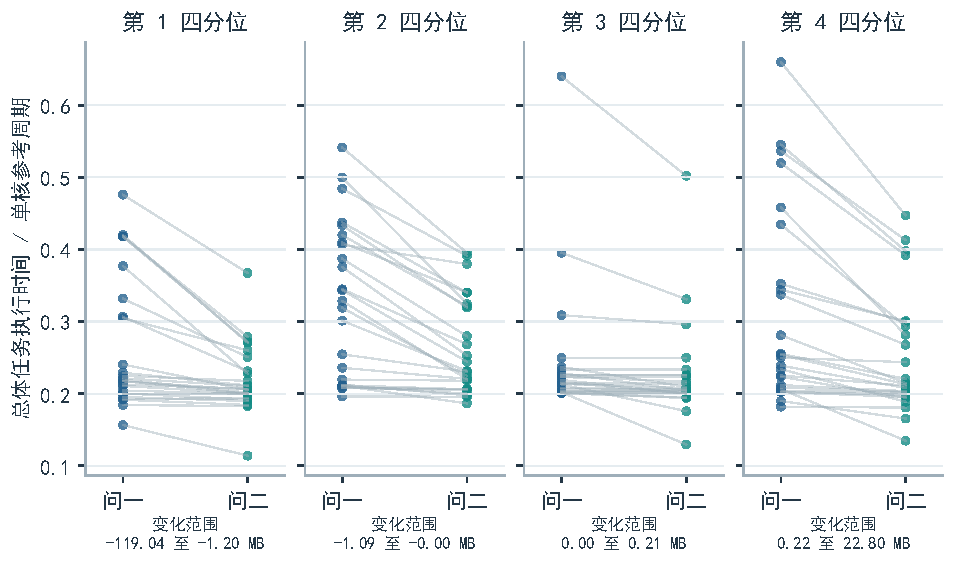
\includegraphics[width=.94\textwidth]{../求解/问题二/图片/q2_copy.pdf}
\caption{按额外 COPY 量变化分组的逐图周期配对}\label{fig:q2_copy}
\end{figure}

存储代价尤其需要与边界收益并看。第一问五核有 88 图无自动换出，第二问为 74 图；第二问五核自动换出新增 COPY 字节的逐图均值为 $2645062.08$ B，高于第一问的 $206080.96$ B。这与更长的同核驻留期相容，却不能仅凭汇总量断言每个图都由容量成为瓶颈。两张第二问周期略长的图分别为图 72 和图 79，其第一、二问五核周期为 $4775553/4781658$ 与 $5985137/6007992$；二者的第二问额外 COPY 字节反而都更少。因此，边界搬运缩减并非 总体任务执行时间 改善的充分条件，还需考虑关键路径、Pipe 排队、活跃缓冲和 DDR 发射时机。

\subsubsection{来源记录与结论边界}
图~\ref{fig:q2_sources} 汇总第二问实际候选来源的调用和周期改善记录。结构来源完成评价 $15656$ 次，其中 $740$ 次带来周期改善；基础来源为 $8589$ 次及 $443$ 次，驻留来源为 $8819$ 次及 $353$ 次。来源调用数和改善数反映搜索过程中各候选被提出、准入与评价后的观察结果，并非关闭其他来源后重跑得到的严格消融。不同来源会相继改变同一当前方案，也面对不同图结构和剩余预算，故不能由改善率单独排序其因果贡献。
\begin{figure}[H]\centering
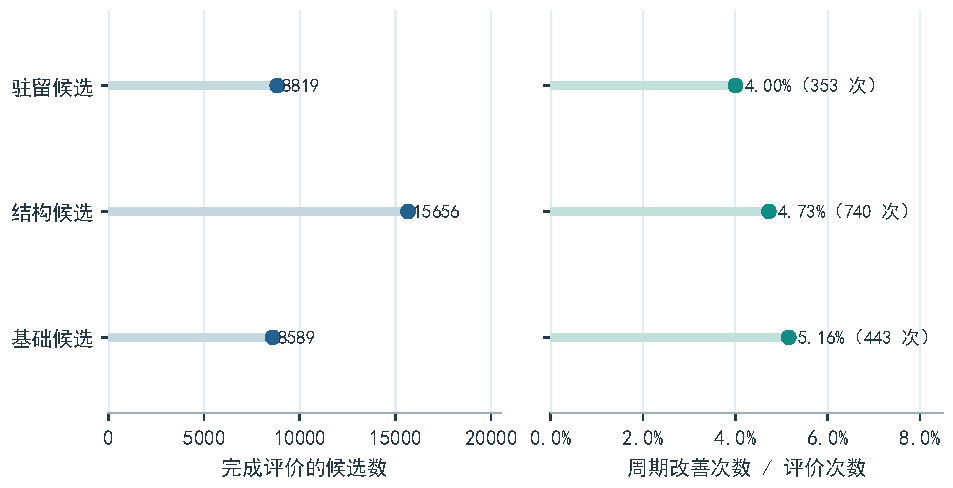
\includegraphics[width=.94\textwidth]{../求解/问题二/图片/q2_sources.pdf}
\caption{第二问候选来源的调用与周期改善记录}\label{fig:q2_sources}
\end{figure}

综合逐图周期、COPY 量和存储记录，第二问的主要机会来自同核跨子图复用与更细的跨核释放，但两者同时改变并行性和片上驻留压力。完整执行评价确保所保留方案满足真实任务、容量、流水线与带宽条件；下界只提供可证明的质量范围。下一问在本问核心级 Task 基础上加入共享只读缓存，需进一步把逻辑 COPY 请求量与实际 DDR 服务量区分。
